%-----------------------------------------------------------------------------
%
%               Template for sigplanconf LaTeX Class
%
% Name:         sigplanconf-template.tex
%
% Purpose:      A template for sigplanconf.cls, which is a LaTeX 2e class
%               file for SIGPLAN conference proceedings.
%
% Guide:        Refer to "Author's Guide to the ACM SIGPLAN Class,"
%               sigplanconf-guide.pdf
%
% Author:       Paul C. Anagnostopoulos
%               Windfall Software
%               978 371-2316
%               paul@windfall.com
%
% Created:      15 February 2005
%
%-----------------------------------------------------------------------------


\documentclass[preprint]{sigplanconf}

% The following \documentclass options may be useful:

% preprint      Remove this option only once the paper is in final form.
% 10pt          To set in 10-point type instead of 9-point.
% 11pt          To set in 11-point type instead of 9-point.
% authoryear    To obtain author/year citation style instead of numeric.

\let\program\undefined % \program from acmtras2e conflicts with our program

\usepackage{amsmath}
\usepackage{program}
\usepackage{graphicx}

\begin{document}

\special{papersize=8.5in,11in}
\setlength{\pdfpageheight}{\paperheight}
\setlength{\pdfpagewidth}{\paperwidth}

\conferenceinfo{Workshop on Programming Models for SIMD/Vector Processing - WPMVP'15}{February 7--8, 2015, San Francisco, CA, USA} 
\copyrightyear{2015} 
\copyrightdata{978-1-nnnn-nnnn-n/15/2} 
\doi{nnnnnnn.nnnnnnn}

% Uncomment one of the following two, if you are not going for the 
% traditional copyright transfer agreement.

%\exclusivelicense                % ACM gets exclusive license to publish, 
                                  % you retain copyright

%\permissiontopublish             % ACM gets nonexclusive license to publish
                                  % (paid open-access papers, 
                                  % short abstracts)

\titlebanner{DRAFT}        % These are ignored unless
\preprintfooter{SIMD in JavaScript via C++ and Emscripten}   % 'preprint' option specified.

\title{SIMD in JavaScript via C++ and Emscripten}
% \subtitle{Subtitle Text, if any}

\authorinfo{Peter Jensen}
           {Intel Corporation}
           {peter.jensen@intel.com}
\authorinfo{John McCutchan}
           {Google Inc.}
           {johnmccutchan@google.com}
\authorinfo{Ivan Jibaja}
           {Intel Corporation}
           {ivan.jibaja@intel.com}
\authorinfo{Dan Gohman}
           {Mozilla}
           {sunfish@mozilla.com}
\authorinfo{Ningxin Hu}
           {Intel Corporation}
           {ningxin.hu@intel.com}

\maketitle

\begin{abstract}
This is the text of the abstract.
\end{abstract}

%\category{CR-number}{subcategory}{third-level}

% general terms are not compulsory anymore, 
% you may leave them out
%\terms
%term1, term2

%\keywords
%keyword1, keyword2

\section{Introduction}

We'll explore the use of Mozilla's Emscripten to compile C++ benchmarks, that has use of SIMD intrinsics,
into JavaScript.  This was recently made possible by the SIMD.JS primitives introduced in
JavaScript VM prototypes for Chromium and Firefox as well as extensions to the Emscripten 
compiler.  Emscripten will correctly translate a subset of available C++ SIMD x86 intrinsics into corresponding operations defined in SIMD.JS.
The JavaScript benchmarks associated with the SIMD.JS primitives were converted to C++ by hand,
and then automatically converted back into JavaScript using the Emscripten compiler.

\section{SIMD.JS}

\begin{figure}
\begin{small}
\begin{program}[style=tt, number=true]
fu\tab{}nction average(data) \{
  var sum = new SIMD.float32x4.splat(0.0);
  fo\tab{}r (var i = 0; i < data.length; i++) \{
    sum = SIMD.float32x4.add(sum, data[i]);\untab{}
  \}
  var total = sum.x + sum.y + sum.z + sum.w;
  return total / (data.length * 4);\untab{}
\}
\end{program}
\end{small}
\caption{Finding the average of an array of numbers in JavaScript using SIMD.}
\label{fig:simd-average}
\end{figure}

\begin{figure}
\begin{center}
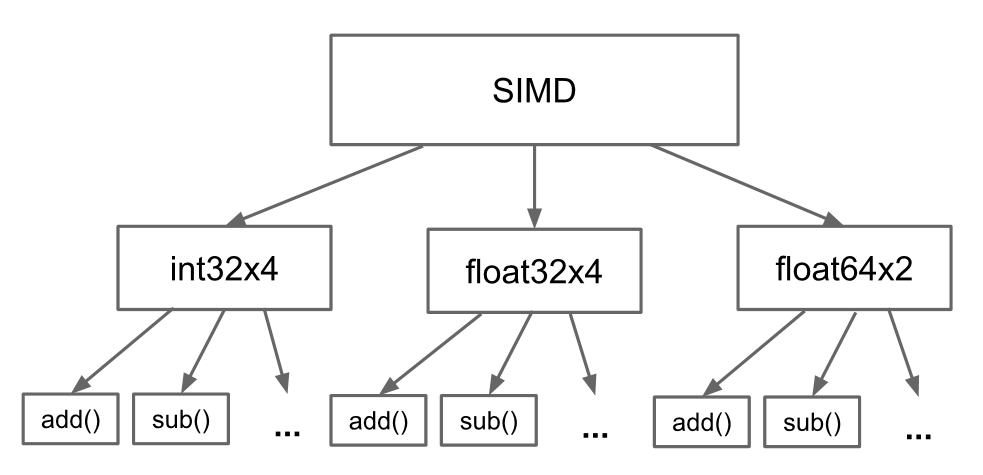
\includegraphics[width=0.5\textwidth]{figures/hierarchy.png}
\end{center}
\caption{SIMD.JS object hierarchy}
\label{fig:hierarchy}
\end{figure}

\section{Emscripten}

\section{Compiling x86 C++ SIMD intrinsics}

\section{Benchmarks}

\section{Results}

\section{Summary}

\appendix
\section{Appendix Title}

This is the text of the appendix, if you need one.

\acks

Acknowledgments, if needed.

% We recommend abbrvnat bibliography style.

\bibliographystyle{abbrvnat}

% The bibliography should be embedded for final submission.

\begin{thebibliography}{}
\softraggedright

\bibitem[Smith et~al.(2009)Smith, Jones]{smith02}
P. Q. Smith, and X. Y. Jones. ...reference text...

\end{thebibliography}


\end{document}

%                       Revision History
%                       -------- -------
%  Date         Person  Ver.    Change
%  ----         ------  ----    ------

%  2013.06.29   TU      0.1--4  comments on permission/copyright notices

